\documentclass[12pt]{article}

\usepackage{listings}
\usepackage{color}
\usepackage{graphicx}
\usepackage[margin=0.7in]{geometry}

\title{ Telecom Software Lab}
\date{12-09-2017}
\author{MOHIT VARSHNEY}

\renewcommand\lstlistingname{Quelltext} % Change language of section name

\lstset{ % General setup for the package
	language=Perl,
	basicstyle=\small\sffamily,
	numbers=left,
 	numberstyle=\tiny,
	frame=tb,
	tabsize=4,
	columns=fixed,
	showstringspaces=false,
	showtabs=false,
	keepspaces,
	commentstyle=\color{red},
	keywordstyle=\color{blue}
}



\begin{document}

\begin{titlepage}

	\begin{center}
    \vspace*{0.5 cm}
    
\includegraphics[width=6 cm, height=6 cm]{iitd_logo.png}\\[1.0 cm]
    														 % University Logo
    \textsc{\LARGE Indian Institute of Technology\newline\newline Delhi}
    \\[2.0 cm]                                    	     % University Name
	\textsc{\Large ELP 718}   \\[0.5 cm]				     % Course Code
	\rule{\linewidth}{0.2 mm} \\[0.4 cm]
	{ \huge \bfseries {TELECOM SOFTWARE LAB}}\\
	\rule{\linewidth}{0.2 mm} \\[1.5 cm]
	\end{center}
	
	\begin{flushright}    \large
	\emph{Submitted By:}  \\
	NAME: MOHIT VARSHNEY  \\
    ENTRY NO.: JTM172019   \\
    DATE: 12-09-2017       \\
    ASSIGNMENT NO.: 6
	\end{flushright}
			
\end{titlepage}
  
  
\pagebreak
\tableofcontents
\pagebreak

\pagenumbering{arabic}
\section{Problem Statement 1}
{
Design a parity check and bit oriented framing program such that odd parity is maintained and parity bit is added in the end of the message and The string 0101 is used as the bit string or flag to indicate the end of the frame. The bit stuffing rule is to insert a 0 after each appearance of 010 in the original data. In addition, if the frame ends in 01, a 0 would be stuffed after the 1st 0 in the actual terminating string 0101.

}

\subsection{Assumptions}
{
Data to be entered in Binary format
}

\subsection{Program Structure}
{
\begin{enumerate}
\item Enter a data which is to be transmitted.
\item Calculate numbers of 1 in data and add parity bit maintaining the odd parity.
\item Look for sequence 010 in original data and insert 0 whenever it occurs.
\item If frame ends with 01 then add 0 in end and then terminate all strings with 0101 
\end{enumerate} 
}




\subsection{Input and Output Format}
{
\textbf{Input Format}\\
Enter binary bit data which has to be transmitted.\\
\textbf{Output Format}\\
Print binary bit data with parity bit.\\
Print the modified string received at the other end.

}
\subsection{Test Cases}

\textbf{Sample Input}\\
01010\\
\textbf{Sample Output}\\
010101\\
0100100100101




\subsection{Screenshots}
{
\begin{center}
    \vspace*{0.5 cm}
  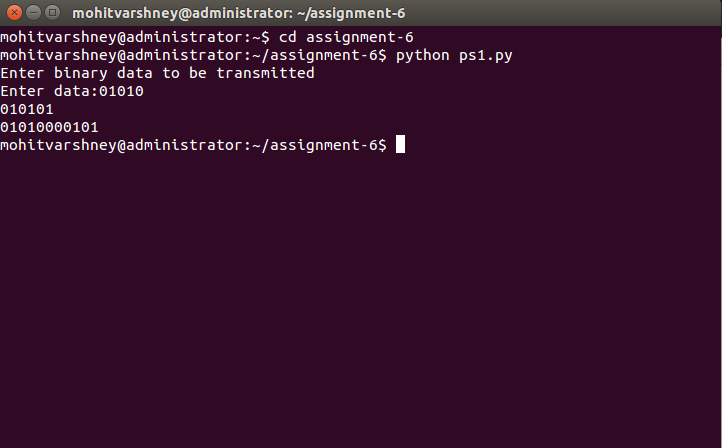
\includegraphics[width=0.9\linewidth]{ps1.png}\\[1.0 cm]
 % \includegraphics[width=0.9\linewidth]{2.png}\\[1.0 cm]
\end{center}    
}



\pagebreak
\section{Problem Statement 2}
\textbf{3X3 Numeric Tic-Tac-Toe} (Use numbers 1 to 9 instead of X’s and O’s)
One player plays with the odd numbers (1, 3, 5, 7, 9) and other player plays with the even numbers (2,4,6,8). All numbers can be used only once. The player who puts down 15 points in a line wins (sum of 3 numbers). Always Player with odd numbers start the game. Once a line contains two numbers whose sum is 15 or greater, there is no way to complete that line, although filling in the remaining cell might be necessary to complete a different line.



\subsection{Assumptions}
{
Line can be horizontal, vertical or diagonal\\
1 $\leq$ Position $\leq$ 9\\
1 $\leq$ Number $\leq$ 9\\
1 $\leq$ Sum $\leq$ 15

}

\subsection{Program Structure}
{
\begin{enumerate}
\item First write a paragraph in a text file.
\item write program to count number of characters in a paragraph
\item Find maximum and minimum occuring characters
\item Change cases of maximum occuring character 
\end{enumerate} 

}


\subsection{Input and Output Format}
{

Print ‘Welcome to the Game!’.    \\
Print whether it is Player 1’s or Player 2’s chance.\\
Get the position and number to be entered from user.\\
Show     tic tac toe with data.\\
Continue till the game gets draw or some player wins and show result.\\
Ask user whether to continue for next game or exit.\\


}


%\subsection{Test Cases}





\subsection{Screenshots}
{
\begin{center}
    \vspace*{0.5 cm}
 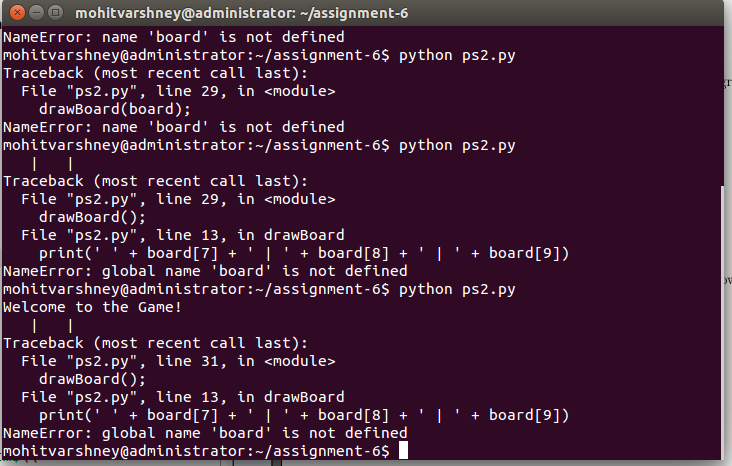
\includegraphics[width=0.9\linewidth]{ps2.png}\\[1.0 cm]
 % \includegraphics[width=0.9\linewidth]{4.png}\\[1.0 cm]
\end{center}    
}

\section{Bibliography}
{
$https://www.tutorialspoint.com/python/python_lists.htm$\\
$https://www.tutorialspoint.com/python/python_loops.htm$\\

}
\newpage

\section{Annexure}
\begin{itemize}

\item\lstinputlisting[language=python, frame = single]{ps1.py}
\item\lstinputlisting[language=python, frame = single]{ps2.py}
%\item\lstinputlisting[language=C, frame = single]{server2.c}
%\item\lstinputlisting[language=C, frame = single]{client2.c}



\end{itemize}
\end{document}